\documentclass[12pt]{article}

\usepackage{amsmath, amssymb}
\usepackage[margin=1in]{geometry}
\usepackage{helvet}
\renewcommand{\familydefault}{\sfdefault}
\def\newrule#1#2#3{\begin{center}
    {#1} \\
    \line(1,0){300} {}{}{}{}{}{}{} [{#3}]\\
    {#2}
\end{center}}

\begin{document}
\def\assignment{Homework 04}

\pagenumbering{gobble}
\noindent{\large COSC 4200 \hfill Name: \underline{Jacob Tuttle} \\ Computability and Complexity}
\begin{center}
    {\Large \assignment} \\ \textbf{\today}
\end{center}

% Question 1 (50 pts)
\begin{enumerate}
  \item \begin{enumerate}
    \item This DFA counts the number of 0s until the acceptance condition is met. At that point, any further input will always result in an accepted state, so it simply reads through the remaining inputs.
      \begin{center}
      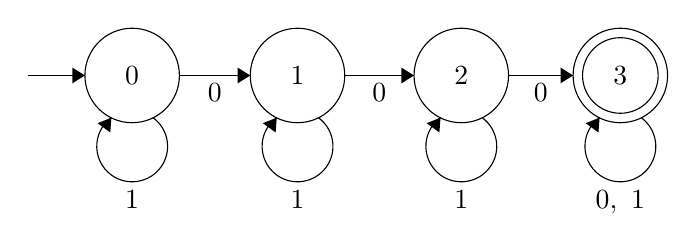
\begin{tikzpicture}[scale=0.2]
      \tikzstyle{every node}+=[inner sep=0pt]
      \draw [black] (9.3,-8) circle (3);
      \draw (9.3,-8) node {$0$};
      \draw [black] (19.8,-8) circle (3);
      \draw (19.8,-8) node {$1$};
      \draw [black] (30.2,-8) circle (3);
      \draw (30.2,-8) node {$2$};
      \draw [black] (40.3,-8) circle (3);
      \draw (40.3,-8) node {$3$};
      \draw [black] (40.3,-8) circle (2.4);
      \draw [black] (2.7,-8) -- (6.3,-8);
      \fill [black] (6.3,-8) -- (5.5,-7.5) -- (5.5,-8.5);
      \draw [black] (10.623,-10.68) arc (54:-234:2.25);
      \draw (9.3,-15.25) node [below] {$1$};
      \fill [black] (7.98,-10.68) -- (7.1,-11.03) -- (7.91,-11.62);
      \draw [black] (12.3,-8) -- (16.8,-8);
      \fill [black] (16.8,-8) -- (16,-7.5) -- (16,-8.5);
      \draw (14.55,-8.5) node [below] {$0$};
      \draw [black] (22.8,-8) -- (27.2,-8);
      \fill [black] (27.2,-8) -- (26.4,-7.5) -- (26.4,-8.5);
      \draw (25,-8.5) node [below] {$0$};
      \draw [black] (33.2,-8) -- (37.3,-8);
      \fill [black] (37.3,-8) -- (36.5,-7.5) -- (36.5,-8.5);
      \draw (35.25,-8.5) node [below] {$0$};
      \draw [black] (41.623,-10.68) arc (54:-234:2.25);
      \draw (40.3,-15.25) node [below] {$0,\mbox{ }1$};
      \fill [black] (38.98,-10.68) -- (38.1,-11.03) -- (38.91,-11.62);
      \draw [black] (21.123,-10.68) arc (54:-234:2.25);
      \draw (19.8,-15.25) node [below] {$1$};
      \fill [black] (18.48,-10.68) -- (17.6,-11.03) -- (18.41,-11.62);
      \draw [black] (31.523,-10.68) arc (54:-234:2.25);
      \draw (30.2,-15.25) node [below] {$1$};
      \fill [black] (28.88,-10.68) -- (28,-11.03) -- (28.81,-11.62);
      \end{tikzpicture}
      \end{center}

    \item This DFA counts the number of 1s present within the input word and will accept the word when there are exactly two 1s within the word. After 3 1s are read, it simply reads through the rest of the word and remains in a failure state.
      \begin{center}
      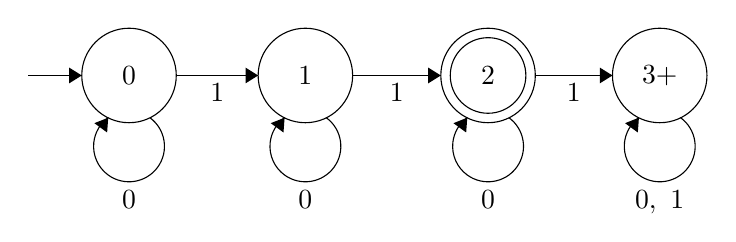
\begin{tikzpicture}[scale=0.2]
      \tikzstyle{every node}+=[inner sep=0pt]
      \draw [black] (9.3,-9.2) circle (3);
      \draw (9.3,-9.2) node {$0$};
      \draw [black] (20.5,-9.2) circle (3);
      \draw (20.5,-9.2) node {$1$};
      \draw [black] (32.1,-9.2) circle (3);
      \draw (32.1,-9.2) node {$2$};
      \draw [black] (32.1,-9.2) circle (2.4);
      \draw [black] (43,-9.2) circle (3);
      \draw (43,-9.2) node {$3+$};
      \draw [black] (12.3,-9.2) -- (17.5,-9.2);
      \fill [black] (17.5,-9.2) -- (16.7,-8.7) -- (16.7,-9.7);
      \draw (14.9,-9.7) node [below] {$1$};
      \draw [black] (23.5,-9.2) -- (29.1,-9.2);
      \fill [black] (29.1,-9.2) -- (28.3,-8.7) -- (28.3,-9.7);
      \draw (26.3,-9.7) node [below] {$1$};
      \draw [black] (35.1,-9.2) -- (40,-9.2);
      \fill [black] (40,-9.2) -- (39.2,-8.7) -- (39.2,-9.7);
      \draw (37.55,-9.7) node [below] {$1$};
      \draw [black] (10.623,-11.88) arc (54:-234:2.25);
      \draw (9.3,-16.45) node [below] {$0$};
      \fill [black] (7.98,-11.88) -- (7.1,-12.23) -- (7.91,-12.82);
      \draw [black] (21.823,-11.88) arc (54:-234:2.25);
      \draw (20.5,-16.45) node [below] {$0$};
      \fill [black] (19.18,-11.88) -- (18.3,-12.23) -- (19.11,-12.82);
      \draw [black] (33.423,-11.88) arc (54:-234:2.25);
      \draw (32.1,-16.45) node [below] {$0$};
      \fill [black] (30.78,-11.88) -- (29.9,-12.23) -- (30.71,-12.82);
      \draw [black] (44.323,-11.88) arc (54:-234:2.25);
      \draw (43,-16.45) node [below] {$0,\mbox{ }1$};
      \fill [black] (41.68,-11.88) -- (40.8,-12.23) -- (41.61,-12.82);
      \draw [black] (2.9,-9.2) -- (6.3,-9.2);
      \fill [black] (6.3,-9.2) -- (5.5,-8.7) -- (5.5,-9.7);
      \end{tikzpicture}
      \end{center}

    \item First, the DFA will ensure that the 01 prefix is within the string. If it reads a different set of first two characters, it will move to, and terminate in, the state labelled "Fail." Otherwise, it will read through the rest of the word, switching between the acceptance state and a non-accepting state until it reaches the end of the word and has checked if 0 is the last character in the word.
      \begin{center}
      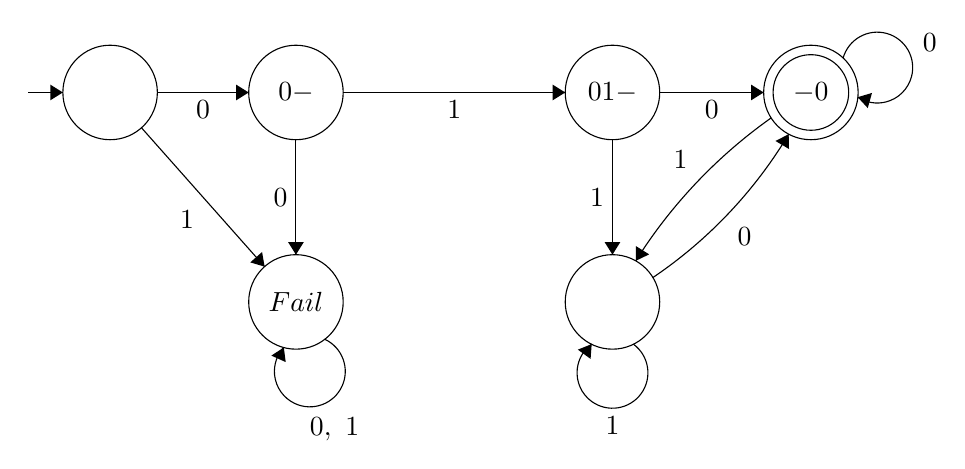
\begin{tikzpicture}[scale=0.2]
      \tikzstyle{every node}+=[inner sep=0pt]
      \draw [black] (8.2,-9) circle (3);
      \draw [black] (20,-9) circle (3);
      \draw (20,-9) node {$0-$};
      \draw [black] (40.1,-9) circle (3);
      \draw (40.1,-9) node {$01-$};
      \draw [black] (52.7,-9) circle (3);
      \draw (52.7,-9) node {$-0$};
      \draw [black] (52.7,-9) circle (2.4);
      \draw [black] (40.1,-22.3) circle (3);
      \draw [black] (20,-22.3) circle (3);
      \draw (20,-22.3) node {$Fail$};
      \draw [black] (3,-9) -- (5.2,-9);
      \fill [black] (5.2,-9) -- (4.4,-8.5) -- (4.4,-9.5);
      \draw [black] (11.2,-9) -- (17,-9);
      \fill [black] (17,-9) -- (16.2,-8.5) -- (16.2,-9.5);
      \draw (14.1,-9.5) node [below] {$0$};
      \draw [black] (23,-9) -- (37.1,-9);
      \fill [black] (37.1,-9) -- (36.3,-8.5) -- (36.3,-9.5);
      \draw (30.05,-9.5) node [below] {$1$};
      \draw [black] (43.1,-9) -- (49.7,-9);
      \fill [black] (49.7,-9) -- (48.9,-8.5) -- (48.9,-9.5);
      \draw (46.4,-9.5) node [below] {$0$};
      \draw [black] (54.745,-6.821) arc (164.55605:-123.44395:2.25);
      \draw (59.78,-5.81) node [right] {$0$};
      \fill [black] (55.67,-9.3) -- (56.31,-9.99) -- (56.58,-9.03);
      \draw [black] (41.578,-19.691) arc (147.79395:125.30236:32.046);
      \fill [black] (41.58,-19.69) -- (42.43,-19.28) -- (41.58,-18.75);
      \draw (44.9,-13.26) node [left] {$1$};
      \draw [black] (51.293,-11.648) arc (-30.95795:-55.94574:28.984);
      \fill [black] (51.29,-11.65) -- (50.45,-12.08) -- (51.31,-12.59);
      \draw (48.01,-18.14) node [right] {$0$};
      \draw [black] (40.1,-12) -- (40.1,-19.3);
      \fill [black] (40.1,-19.3) -- (40.6,-18.5) -- (39.6,-18.5);
      \draw (39.6,-15.65) node [left] {$1$};
      \draw [black] (41.423,-24.98) arc (54:-234:2.25);
      \draw (40.1,-29.55) node [below] {$1$};
      \fill [black] (38.78,-24.98) -- (37.9,-25.33) -- (38.71,-25.92);
      \draw [black] (20,-12) -- (20,-19.3);
      \fill [black] (20,-19.3) -- (20.5,-18.5) -- (19.5,-18.5);
      \draw (19.5,-15.65) node [left] {$0$};
      \draw [black] (10.19,-11.24) -- (18.01,-20.06);
      \fill [black] (18.01,-20.06) -- (17.85,-19.13) -- (17.1,-19.79);
      \draw (13.56,-17.1) node [left] {$1$};
      \draw [black] (21.822,-24.668) arc (65.30993:-222.69007:2.25);
      \draw (22.45,-29.59) node [below] {$0,\mbox{ }1$};
      \fill [black] (19.23,-25.19) -- (18.44,-25.71) -- (19.35,-26.12);
      \end{tikzpicture}
      \end{center}

    \item This DFA will progress through states labeled with the length of the word until it reaches the end of the word. If the length of the word is between 3 and 5 inclusively, it will end in an acceptance state, but if the word length is six or more characters, it will simply remain in the 6+ state until the word has been fully read.
      \begin{center}
      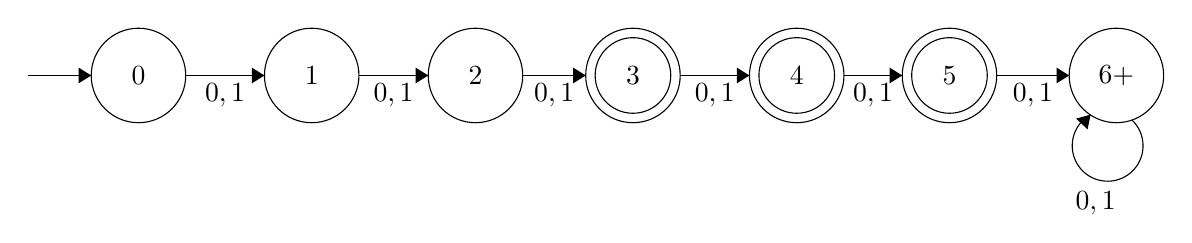
\begin{tikzpicture}[scale=0.2]
      \tikzstyle{every node}+=[inner sep=0pt]
      \draw [black] (9.5,-10) circle (3);
      \draw (9.5,-10) node {$0$};
      \draw [black] (20.5,-10) circle (3);
      \draw (20.5,-10) node {$1$};
      \draw [black] (30.9,-10) circle (3);
      \draw (30.9,-10) node {$2$};
      \draw [black] (40.9,-10) circle (3);
      \draw (40.9,-10) node {$3$};
      \draw [black] (40.9,-10) circle (2.4);
      \draw [black] (51.3,-10) circle (3);
      \draw (51.3,-10) node {$4$};
      \draw [black] (51.3,-10) circle (2.4);
      \draw [black] (61,-10) circle (3);
      \draw (61,-10) node {$5$};
      \draw [black] (61,-10) circle (2.4);
      \draw [black] (71.6,-10) circle (3);
      \draw (71.6,-10) node {$6+$};
      \draw [black] (12.5,-10) -- (17.5,-10);
      \fill [black] (17.5,-10) -- (16.7,-9.5) -- (16.7,-10.5);
      \draw (15,-10.5) node [below] {$0,1$};
      \draw [black] (23.5,-10) -- (27.9,-10);
      \fill [black] (27.9,-10) -- (27.1,-9.5) -- (27.1,-10.5);
      \draw (25.7,-10.5) node [below] {$0,1$};
      \draw [black] (33.9,-10) -- (37.9,-10);
      \fill [black] (37.9,-10) -- (37.1,-9.5) -- (37.1,-10.5);
      \draw (35.9,-10.5) node [below] {$0,1$};
      \draw [black] (43.9,-10) -- (48.3,-10);
      \fill [black] (48.3,-10) -- (47.5,-9.5) -- (47.5,-10.5);
      \draw (46.1,-10.5) node [below] {$0,1$};
      \draw [black] (54.3,-10) -- (58,-10);
      \fill [black] (58,-10) -- (57.2,-9.5) -- (57.2,-10.5);
      \draw (56.15,-10.5) node [below] {$0,1$};
      \draw [black] (2.5,-10) -- (6.5,-10);
      \fill [black] (6.5,-10) -- (5.7,-9.5) -- (5.7,-10.5);
      \draw [black] (64,-10) -- (68.6,-10);
      \fill [black] (68.6,-10) -- (67.8,-9.5) -- (67.8,-10.5);
      \draw (66.3,-10.5) node [below] {$0,1$};
      \draw [black] (72.58,-12.823) arc (46.87498:-241.12502:2.25);
      \draw (70.28,-17.36) node [below] {$0,1$};
      \fill [black] (69.96,-12.49) -- (69.04,-12.74) -- (69.77,-13.42);
      \end{tikzpicture}
      \end{center}

    \item This DFA works by constructing a circuit that is the length of the least common multiple of 2 and 3, namely 6, states. The states, in order from the input state represent the length being divisible by: both 2 and 3, neither, only 2, only 3, only 2, neither, and both 2 and 3. Since this pattern repeats as length grows to infinity, however long the word is will be accurately counted and then properly divided by this DFA. Also note, all state transitions will transition on an input of 'a' but are not marked as such since only one input character is possible in the given alphabet.
      \begin{center}
      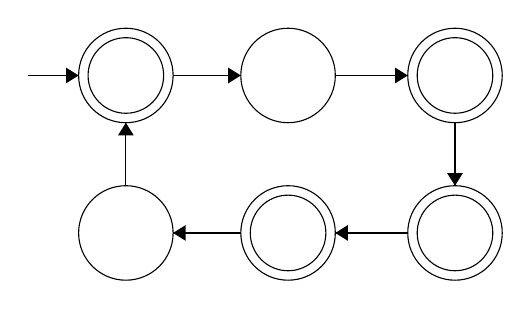
\begin{tikzpicture}[scale=0.2]
      \tikzstyle{every node}+=[inner sep=0pt]
      \draw [black] (7.2,-7.9) circle (3);
      \draw [black] (7.2,-7.9) circle (2.4);
      \draw [black] (17.5,-7.9) circle (3);
      \draw [black] (28.1,-7.9) circle (3);
      \draw [black] (28.1,-7.9) circle (2.4);
      \draw [black] (28.1,-17.9) circle (3);
      \draw [black] (28.1,-17.9) circle (2.4);
      \draw [black] (17.5,-17.9) circle (3);
      \draw [black] (17.5,-17.9) circle (2.4);
      \draw [black] (7.2,-17.9) circle (3);
      \draw [black] (10.2,-7.9) -- (14.5,-7.9);
      \fill [black] (14.5,-7.9) -- (13.7,-7.4) -- (13.7,-8.4);
      \draw [black] (20.5,-7.9) -- (25.1,-7.9);
      \fill [black] (25.1,-7.9) -- (24.3,-7.4) -- (24.3,-8.4);
      \draw [black] (1,-7.9) -- (4.2,-7.9);
      \fill [black] (4.2,-7.9) -- (3.4,-7.4) -- (3.4,-8.4);
      \draw [black] (28.1,-10.9) -- (28.1,-14.9);
      \fill [black] (28.1,-14.9) -- (28.6,-14.1) -- (27.6,-14.1);
      \draw [black] (25.1,-17.9) -- (20.5,-17.9);
      \fill [black] (20.5,-17.9) -- (21.3,-18.4) -- (21.3,-17.4);
      \draw [black] (14.5,-17.9) -- (10.2,-17.9);
      \fill [black] (10.2,-17.9) -- (11,-18.4) -- (11,-17.4);
      \draw [black] (7.2,-14.9) -- (7.2,-10.9);
      \fill [black] (7.2,-10.9) -- (6.7,-11.7) -- (7.7,-11.7);
      \end{tikzpicture}
      \end{center}

    \item This DFA keeps track of the last two read characters. If they are different, and the entire word has been read, then the word ends with either ba or ab. Otherwise, the DFA will finish in a non-accepting state.
      \begin{center}
      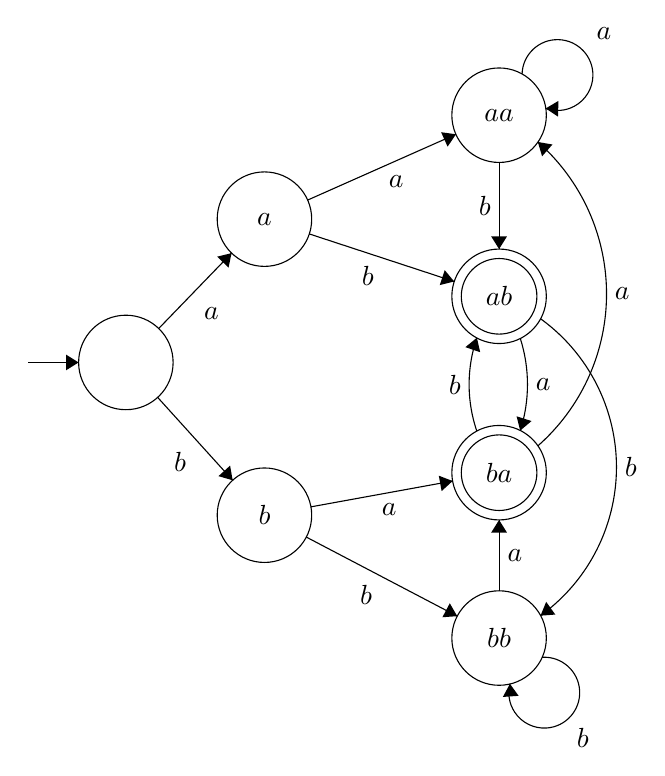
\begin{tikzpicture}[scale=0.2]
      \tikzstyle{every node}+=[inner sep=0pt]
      \draw [black] (8.4,-22.3) circle (3);
      \draw [black] (17.2,-13.2) circle (3);
      \draw (17.2,-13.2) node {$a$};
      \draw [black] (17.2,-32) circle (3);
      \draw (17.2,-32) node {$b$};
      \draw [black] (32.1,-6.6) circle (3);
      \draw (32.1,-6.6) node {$aa$};
      \draw [black] (32.1,-18.1) circle (3);
      \draw (32.1,-18.1) node {$ab$};
      \draw [black] (32.1,-18.1) circle (2.4);
      \draw [black] (32.1,-29.3) circle (3);
      \draw (32.1,-29.3) node {$ba$};
      \draw [black] (32.1,-29.3) circle (2.4);
      \draw [black] (32.1,-39.8) circle (3);
      \draw (32.1,-39.8) node {$bb$};
      \draw [black] (10.49,-20.14) -- (15.11,-15.36);
      \fill [black] (15.11,-15.36) -- (14.2,-15.58) -- (14.92,-16.28);
      \draw (13.33,-19.22) node [right] {$a$};
      \draw [black] (10.42,-24.52) -- (15.18,-29.78);
      \fill [black] (15.18,-29.78) -- (15.02,-28.85) -- (14.28,-29.52);
      \draw (12.26,-28.61) node [left] {$b$};
      \draw [black] (19.94,-11.99) -- (29.36,-7.81);
      \fill [black] (29.36,-7.81) -- (28.42,-7.68) -- (28.83,-8.6);
      \draw (25.57,-10.41) node [below] {$a$};
      \draw [black] (20.05,-14.14) -- (29.25,-17.16);
      \fill [black] (29.25,-17.16) -- (28.65,-16.44) -- (28.33,-17.39);
      \draw (23.77,-16.19) node [below] {$b$};
      \draw [black] (20.15,-31.47) -- (29.15,-29.83);
      \fill [black] (29.15,-29.83) -- (28.27,-29.49) -- (28.45,-30.47);
      \draw (25.12,-31.24) node [below] {$a$};
      \draw [black] (19.86,-33.39) -- (29.44,-38.41);
      \fill [black] (29.44,-38.41) -- (28.97,-37.59) -- (28.5,-38.48);
      \draw (23.66,-36.4) node [below] {$b$};
      \draw [black] (30.688,-26.668) arc (-161.14367:-198.85633:9.184);
      \fill [black] (30.69,-20.73) -- (29.96,-21.33) -- (30.9,-21.65);
      \draw (29.7,-23.7) node [left] {$b$};
      \draw [black] (33.444,-20.769) arc (17.77536:-17.77536:9.602);
      \fill [black] (33.44,-26.63) -- (34.16,-26.02) -- (33.21,-25.72);
      \draw (34.4,-23.7) node [right] {$a$};
      \draw [black] (32.1,-36.8) -- (32.1,-32.3);
      \fill [black] (32.1,-32.3) -- (31.6,-33.1) -- (32.6,-33.1);
      \draw (32.6,-34.55) node [right] {$a$};
      \draw [black] (34.827,-41.022) arc (93.59136:-194.40864:2.25);
      \draw (37.41,-45.49) node [below] {$b$};
      \fill [black] (32.79,-42.71) -- (32.34,-43.54) -- (33.34,-43.47);
      \draw [black] (33.559,-3.992) arc (178.50852:-109.49148:2.25);
      \draw (38.26,-1.42) node [right] {$a$};
      \fill [black] (35.06,-6.17) -- (35.84,-6.69) -- (35.87,-5.69);
      \draw [black] (34.562,-8.303) arc (48.64309:-48.64309:12.853);
      \fill [black] (34.56,-8.3) -- (34.83,-9.21) -- (35.49,-8.46);
      \draw (39.42,-17.95) node [right] {$a$};
      \draw [black] (34.731,-19.524) arc (54.18503:-54.18503:11.624);
      \fill [black] (34.73,-38.38) -- (35.67,-38.31) -- (35.09,-37.5);
      \draw (40.05,-28.95) node [right] {$b$};
      \draw [black] (32.1,-9.6) -- (32.1,-15.1);
      \fill [black] (32.1,-15.1) -- (32.6,-14.3) -- (31.6,-14.3);
      \draw (31.6,-12.35) node [left] {$b$};
      \draw [black] (2.2,-22.3) -- (5.4,-22.3);
      \fill [black] (5.4,-22.3) -- (4.6,-21.8) -- (4.6,-22.8);
      \end{tikzpicture}
      \end{center}

    \item This DFA keeps track of substrings that begin to look like the non-accepting substring 110. If That substring is recognized within the DFA, it moves to an always non-accepting state. Otherwise, regardless of which state the DFA is in, it will accept the word since the substring does not appear within it.
      \begin{center}
      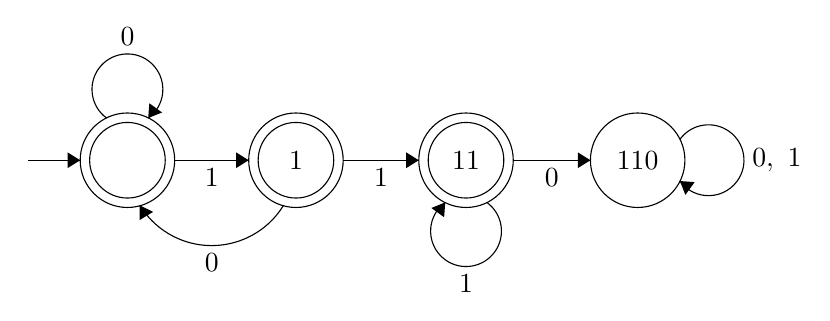
\begin{tikzpicture}[scale=0.2]
      \tikzstyle{every node}+=[inner sep=0pt]
      \draw [black] (9.6,-11) circle (3);
      \draw [black] (9.6,-11) circle (2.4);
      \draw [black] (20.3,-11) circle (3);
      \draw (20.3,-11) node {$1$};
      \draw [black] (20.3,-11) circle (2.4);
      \draw [black] (31.1,-11) circle (3);
      \draw (31.1,-11) node {$11$};
      \draw [black] (31.1,-11) circle (2.4);
      \draw [black] (42,-11) circle (3);
      \draw (42,-11) node {$110$};
      \draw [black] (3.3,-11) -- (6.6,-11);
      \fill [black] (6.6,-11) -- (5.8,-10.5) -- (5.8,-11.5);
      \draw [black] (44.68,-9.677) arc (144:-144:2.25);
      \draw (49.25,-11) node [right] {$0,\mbox{ }1$};
      \fill [black] (44.68,-12.32) -- (45.03,-13.2) -- (45.62,-12.39);
      \draw [black] (34.1,-11) -- (39,-11);
      \fill [black] (39,-11) -- (38.2,-10.5) -- (38.2,-11.5);
      \draw (36.55,-11.5) node [below] {$0$};
      \draw [black] (23.3,-11) -- (28.1,-11);
      \fill [black] (28.1,-11) -- (27.3,-10.5) -- (27.3,-11.5);
      \draw (25.7,-11.5) node [below] {$1$};
      \draw [black] (12.6,-11) -- (17.3,-11);
      \fill [black] (17.3,-11) -- (16.5,-10.5) -- (16.5,-11.5);
      \draw (14.95,-11.5) node [below] {$1$};
      \draw [black] (19.517,-13.856) arc (-31.39208:-148.60792:5.35);
      \fill [black] (10.38,-13.86) -- (10.37,-14.8) -- (11.23,-14.28);
      \draw (14.95,-16.92) node [below] {$0$};
      \draw [black] (32.423,-13.68) arc (54:-234:2.25);
      \draw (31.1,-18.25) node [below] {$1$};
      \fill [black] (29.78,-13.68) -- (28.9,-14.03) -- (29.71,-14.62);
      \draw [black] (8.277,-8.32) arc (234:-54:2.25);
      \draw (9.6,-3.75) node [above] {$0$};
      \fill [black] (10.92,-8.32) -- (11.8,-7.97) -- (10.99,-7.38);
      \end{tikzpicture}
      \end{center}

    \item This DFA is best represented by a union of the three DFAs that make it up. These will check that there is at least 1 a, no more than 3 bs, and exactly 1 c. We will define the DFA that combines these three smaller DFAs mathematically. $Q = \{a_ib_jc_k | 0 \leq i \leq 1, 0 \leq j \leq 4, 0 \leq k \leq 2\}$; $\Sigma = \{a, b, c\}$; $\delta$ will be defined in parts below; $a_0b_0c_0$ is the initial state; and $F = \{a_1b_0c_1, a_1b_1c_1, a_1b_2c_1, a_1b_3c_1\}$. \\

    Let $\delta'$ be the function that describes the joint DFA for determining the number of bs and cs. We will define $\delta'$ for all $0 \leq i \leq 3$ as:
    \[\begin{array}{ccc}
      \delta'(b_ic_0, a) = b_ic_0 & \delta'(b_ic_1, a) = b_ic_1 & \delta'(b_ic_2, a) = b_ic_2 \\
      \delta'(b_ic_0, b) = b_{i+1}c_0 & \delta'(b_ic_1, b) = b_{i+1}c_1 & \delta'(b_ic_2, b) = b_{i+1}c_2 \\
      \delta'(b_ic_0, c) = b_ic_1 & \delta'(b_ic_1, c) = b_ic_2 & \delta'(b_ic_2, c) = b_ic_2
    \end{array}\]

    \[\begin{array}{ccc}
      \delta'(b_4c_0, a) = b_4c_0 & \delta'(b_4c_1, a) = b_4c_1 & \delta'(b_4c_2, a) = b_4c_2 \\
      \delta'(b_4c_0, b) = b_4c_0 & \delta'(b_4c_1, b) = b_4c_1 & \delta'(b_4c_2, b) = b_4c_2 \\
      \delta'(b_4c_0, c) = b_4c_1 & \delta'(b_4c_1, c) = b_4c_2 & \delta'(b_4c_2, c) = b_4c_2
    \end{array}\]

    From this definition, we can then combine it with the DFA to count as by piecing togethether this definition of $\delta''$ using a state $b_ic_j$ as $x$
    \[\begin{array}{ccc}
      \delta''(a_0x, a) = a_1\delta'(x, a) & \delta''(a_1x, a) = a_1\delta'(x, a) \\
      \delta''(a_0x, b) = a_0\delta'(x, b) & \delta''(a_1x, b) = a_1\delta'(x, b) \\
      \delta''(a_0x, c) = a_0\delta'(x, c) & \delta''(a_1x, c) = a_1\delta'(x, c)
    \end{array}\]

    For instance, $\delta''(a_1b_0c_0, b) = a_1\delta'(b_0c_0, b) = a_1b_1c_0$. This final result of evaluating $\delta''$ is the transition function $\delta$. Thus, we have a DFA that will end up in an accepting state if there is at least 1 a (represented by the partial state $a_1$), there are at most 3 bs (represented by the inclusions of partial states $b_0$ through $b_3$), and there is exactly 1 c (represented by partial state $c_1$). All other states are excluded from the DFA's set of accepting states since at least one of the three criteria for acceptance would not have been met.

    \item Based on the input character, this DFA will branch into one of two sub-DFAs that measures the parity. They both alternate whenever a 1 is read to oscilate between matching parity and mismatched parity. If the parity matches the first bit, then the DFA will accept.
      \begin{center}
      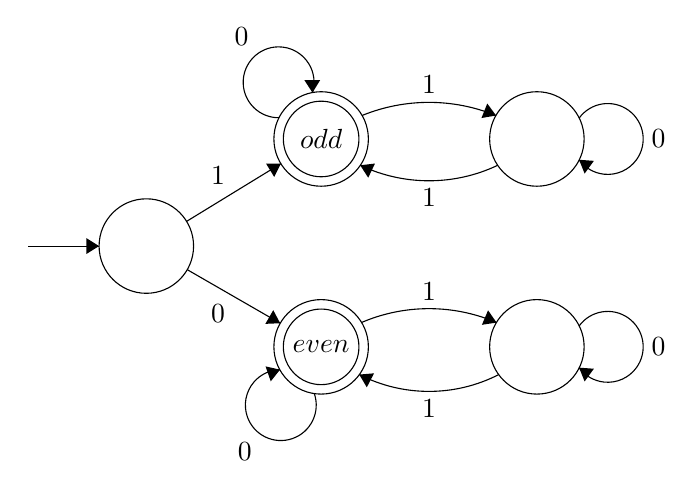
\begin{tikzpicture}[scale=0.2]
      \tikzstyle{every node}+=[inner sep=0pt]
      \draw [black] (9.4,-16.5) circle (3);
      \draw [black] (20.5,-9.7) circle (3);
      \draw (20.5,-9.7) node {$odd$};
      \draw [black] (20.5,-9.7) circle (2.4);
      \draw [black] (20.5,-22.9) circle (3);
      \draw (20.5,-22.9) node {$even$};
      \draw [black] (20.5,-22.9) circle (2.4);
      \draw [black] (34.2,-9.7) circle (3);
      \draw [black] (34.2,-22.9) circle (3);
      \draw [black] (1.9,-16.5) -- (6.4,-16.5);
      \fill [black] (6.4,-16.5) -- (5.6,-16) -- (5.6,-17);
      \draw [black] (11.96,-14.93) -- (17.94,-11.27);
      \fill [black] (17.94,-11.27) -- (17,-11.26) -- (17.52,-12.11);
      \draw (13.95,-12.6) node [above] {$1$};
      \draw [black] (23.094,-8.211) arc (112.22196:67.77804:11.253);
      \fill [black] (31.61,-8.21) -- (31.05,-7.45) -- (30.68,-8.37);
      \draw (27.35,-6.87) node [above] {$1$};
      \draw [black] (12,-18) -- (17.9,-21.4);
      \fill [black] (17.9,-21.4) -- (17.46,-20.57) -- (16.96,-21.44);
      \draw (13.95,-20.2) node [below] {$0$};
      \draw [black] (23.061,-21.355) arc (113.2092:66.7908:10.884);
      \fill [black] (31.64,-21.36) -- (31.1,-20.58) -- (30.71,-21.5);
      \draw (27.35,-19.97) node [above] {$1$};
      \draw [black] (36.88,-21.577) arc (144:-144:2.25);
      \draw (41.45,-22.9) node [right] {$0$};
      \fill [black] (36.88,-24.22) -- (37.23,-25.1) -- (37.82,-24.29);
      \draw [black] (36.88,-8.377) arc (144:-144:2.25);
      \draw (41.45,-9.7) node [right] {$0$};
      \fill [black] (36.88,-11.02) -- (37.23,-11.9) -- (37.82,-11.09);
      \draw [black] (17.834,-8.35) arc (270.8699:-17.1301:2.25);
      \draw (15.45,-3.8) node [above] {$0$};
      \fill [black] (19.95,-6.76) -- (20.44,-5.96) -- (19.44,-5.97);
      \draw [black] (20.062,-25.856) arc (19.30485:-268.69515:2.25);
      \draw (15.66,-28.95) node [below] {$0$};
      \fill [black] (17.89,-24.35) -- (16.97,-24.14) -- (17.3,-25.09);
      \draw [black] (31.783,-24.658) arc (-62.82574:-117.17426:9.708);
      \fill [black] (22.92,-24.66) -- (23.4,-25.47) -- (23.86,-24.58);
      \draw (27.35,-26.23) node [below] {$1$};
      \draw [black] (31.719,-11.368) arc (-64.54557:-115.45443:10.166);
      \fill [black] (22.98,-11.37) -- (23.49,-12.16) -- (23.92,-11.26);
      \draw (27.35,-12.85) node [below] {$1$};
      \end{tikzpicture}
      \end{center}

    \item This DFA will branch into one of three different "paths" to keep track of what the first symbol is. Then, as subsequent letters are read, the DFA will move to an accepting state if the next characters are different than the first one, and it will move to a non-accepting state if the first symbol matches the last read symbol.
      \begin{center}
      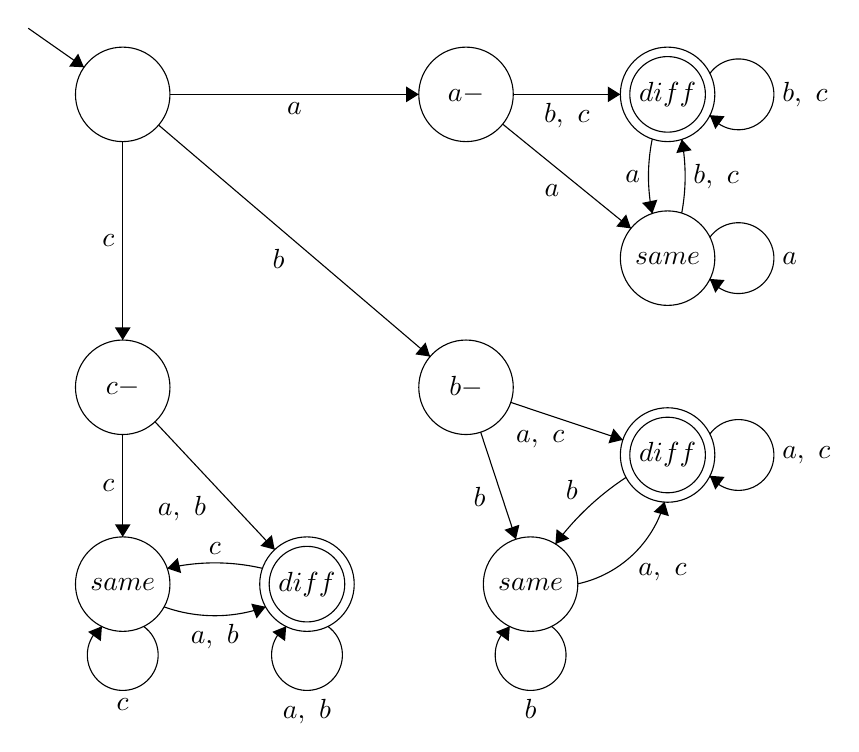
\begin{tikzpicture}[scale=0.2]
      \tikzstyle{every node}+=[inner sep=0pt]
      \draw [black] (12.2,-9.4) circle (3);
      \draw [black] (34,-9.4) circle (3);
      \draw (34,-9.4) node {$a-$};
      \draw [black] (34,-28) circle (3);
      \draw (34,-28) node {$b-$};
      \draw [black] (12.2,-28) circle (3);
      \draw (12.2,-28) node {$c-$};
      \draw [black] (12.2,-40.5) circle (3);
      \draw (12.2,-40.5) node {$same$};
      \draw [black] (23.9,-40.5) circle (3);
      \draw (23.9,-40.5) node {$diff$};
      \draw [black] (23.9,-40.5) circle (2.4);
      \draw [black] (38.1,-40.5) circle (3);
      \draw (38.1,-40.5) node {$same$};
      \draw [black] (46.8,-32.3) circle (3);
      \draw (46.8,-32.3) node {$diff$};
      \draw [black] (46.8,-32.3) circle (2.4);
      \draw [black] (46.8,-9.4) circle (3);
      \draw (46.8,-9.4) node {$diff$};
      \draw [black] (46.8,-9.4) circle (2.4);
      \draw [black] (46.8,-19.8) circle (3);
      \draw (46.8,-19.8) node {$same$};
      \draw [black] (6.2,-5.2) -- (9.74,-7.68);
      \fill [black] (9.74,-7.68) -- (9.37,-6.81) -- (8.8,-7.63);
      \draw [black] (12.2,-12.4) -- (12.2,-25);
      \fill [black] (12.2,-25) -- (12.7,-24.2) -- (11.7,-24.2);
      \draw (11.7,-18.7) node [left] {$c$};
      \draw [black] (14.48,-11.35) -- (31.72,-26.05);
      \fill [black] (31.72,-26.05) -- (31.43,-25.15) -- (30.78,-25.91);
      \draw (22.09,-19.19) node [below] {$b$};
      \draw [black] (15.2,-9.4) -- (31,-9.4);
      \fill [black] (31,-9.4) -- (30.2,-8.9) -- (30.2,-9.9);
      \draw (23.1,-9.9) node [below] {$a$};
      \draw [black] (37,-9.4) -- (43.8,-9.4);
      \fill [black] (43.8,-9.4) -- (43,-8.9) -- (43,-9.9);
      \draw (40.4,-9.9) node [below] {$b,\mbox{ }c$};
      \draw [black] (49.48,-8.077) arc (144:-144:2.25);
      \draw (54.05,-9.4) node [right] {$b,\mbox{ }c$};
      \fill [black] (49.48,-10.72) -- (49.83,-11.6) -- (50.42,-10.79);
      \draw [black] (45.827,-16.971) arc (-168.34089:-191.65911:11.732);
      \fill [black] (45.83,-16.97) -- (46.15,-16.09) -- (45.18,-16.29);
      \draw (45.08,-14.6) node [left] {$a$};
      \draw [black] (36.33,-11.29) -- (44.47,-17.91);
      \fill [black] (44.47,-17.91) -- (44.17,-17.02) -- (43.54,-17.79);
      \draw (39.45,-15.09) node [below] {$a$};
      \draw [black] (47.696,-12.256) arc (10.64397:-10.64397:12.691);
      \fill [black] (47.7,-12.26) -- (47.35,-13.13) -- (48.33,-12.95);
      \draw (48.41,-14.6) node [right] {$b,\mbox{ }c$};
      \draw [black] (49.48,-18.477) arc (144:-144:2.25);
      \draw (54.05,-19.8) node [right] {$a$};
      \fill [black] (49.48,-21.12) -- (49.83,-22) -- (50.42,-21.19);
      \draw [black] (12.2,-31) -- (12.2,-37.5);
      \fill [black] (12.2,-37.5) -- (12.7,-36.7) -- (11.7,-36.7);
      \draw (11.7,-34.25) node [left] {$c$};
      \draw [black] (14.25,-30.19) -- (21.85,-38.31);
      \fill [black] (21.85,-38.31) -- (21.67,-37.38) -- (20.94,-38.07);
      \draw (17.52,-35.72) node [left] {$a,\mbox{ }b$};
      \draw [black] (25.223,-43.18) arc (54:-234:2.25);
      \draw (23.9,-47.75) node [below] {$a,\mbox{ }b$};
      \fill [black] (22.58,-43.18) -- (21.7,-43.53) -- (22.51,-44.12);
      \draw [black] (21.283,-41.941) arc (-70.17194:-109.82806:9.531);
      \fill [black] (21.28,-41.94) -- (20.36,-41.74) -- (20.7,-42.68);
      \draw (18.05,-43.01) node [below] {$a,\mbox{ }b$};
      \draw [black] (15.021,-39.498) arc (103.10988:76.89012:13.353);
      \fill [black] (15.02,-39.5) -- (15.91,-39.8) -- (15.69,-38.83);
      \draw (18.05,-38.65) node [above] {$c$};
      \draw [black] (13.523,-43.18) arc (54:-234:2.25);
      \draw (12.2,-47.75) node [below] {$c$};
      \fill [black] (10.88,-43.18) -- (10,-43.53) -- (10.81,-44.12);
      \draw [black] (36.84,-28.96) -- (43.96,-31.34);
      \fill [black] (43.96,-31.34) -- (43.36,-30.62) -- (43.04,-31.56);
      \draw (38.71,-30.72) node [below] {$a,\mbox{ }c$};
      \draw [black] (34.93,-30.85) -- (37.17,-37.65);
      \fill [black] (37.17,-37.65) -- (37.39,-36.73) -- (36.44,-37.05);
      \draw (35.28,-34.94) node [left] {$b$};
      \draw [black] (39.423,-43.18) arc (54:-234:2.25);
      \draw (38.1,-47.75) node [below] {$b$};
      \fill [black] (36.78,-43.18) -- (35.9,-43.53) -- (36.71,-44.12);
      \draw [black] (46.608,-35.273) arc (-15.4347:-77.95459:7.321);
      \fill [black] (46.61,-35.27) -- (45.91,-35.91) -- (46.88,-36.18);
      \draw (46.48,-39.14) node [below] {$a,\mbox{ }c$};
      \draw [black] (39.677,-37.952) arc (143.37358:123.23713:17.633);
      \fill [black] (39.68,-37.95) -- (40.56,-37.61) -- (39.75,-37.01);
      \draw (40.72,-35.16) node [above] {$b$};
      \draw [black] (49.48,-30.977) arc (144:-144:2.25);
      \draw (54.05,-32.3) node [right] {$a,\mbox{ }c$};
      \fill [black] (49.48,-33.62) -- (49.83,-34.5) -- (50.42,-33.69);
      \end{tikzpicture}
      \end{center}
  \end{enumerate}

  \newpage

  % Problem 2
  \item This DFA will read in the first two characters of the word, $w$ and then continue reading characters. Each of the "arms" of the DFA will look for the substring $w^R$, and if that substring is the end of the input word, accept the input. Otherwise, it will fail since the input doesn't match the construction rules for the language.
    \begin{center}
    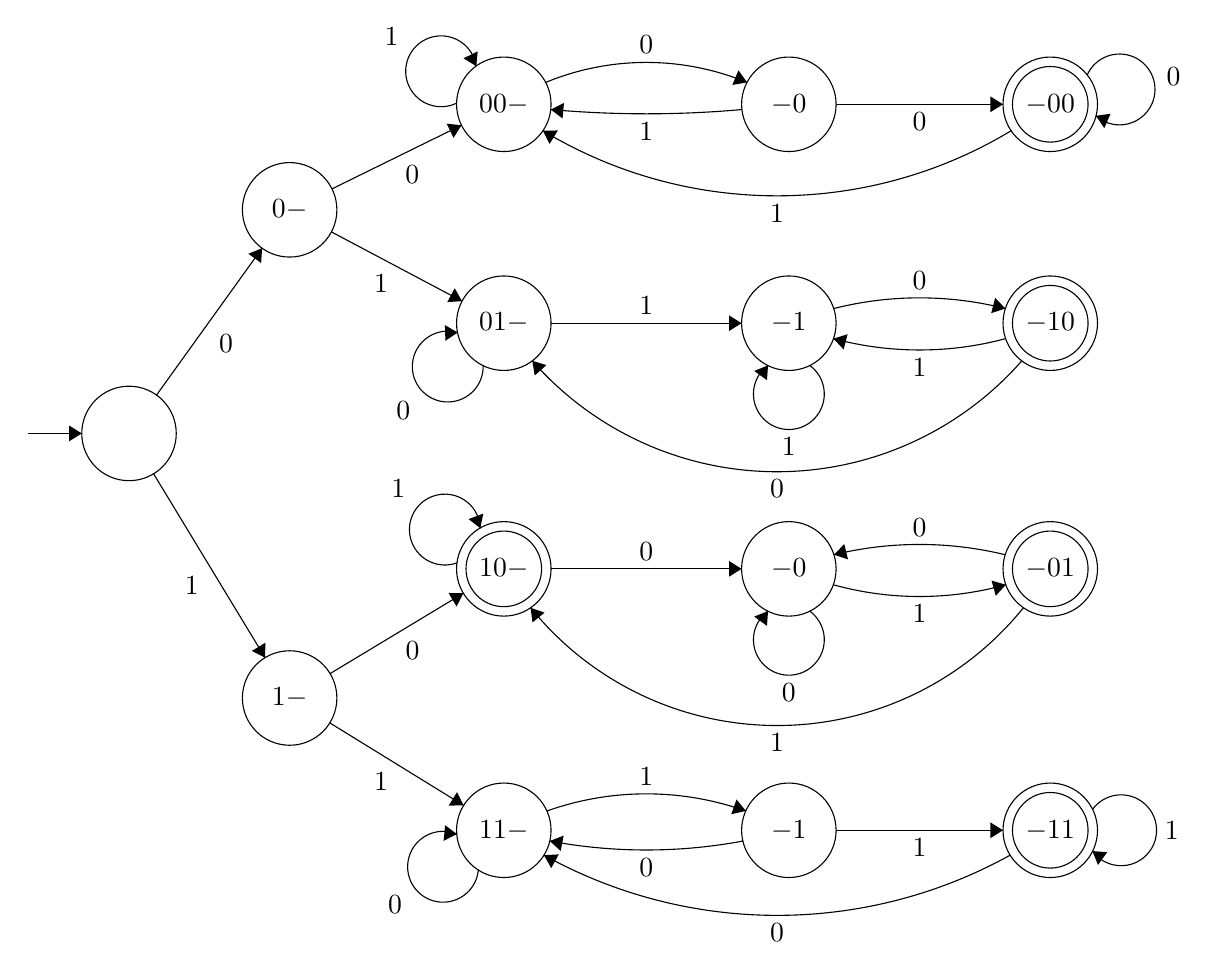
\begin{tikzpicture}[scale=0.2]
    \tikzstyle{every node}+=[inner sep=0pt]
    \draw [black] (8.4,-27.3) circle (3);
    \draw [black] (18.6,-13.1) circle (3);
    \draw (18.6,-13.1) node {$0-$};
    \draw [black] (18.6,-44.1) circle (3);
    \draw (18.6,-44.1) node {$1-$};
    \draw [black] (32.2,-6.4) circle (3);
    \draw (32.2,-6.4) node {$00-$};
    \draw [black] (32.2,-20.3) circle (3);
    \draw (32.2,-20.3) node {$01-$};
    \draw [black] (32.2,-35.9) circle (3);
    \draw (32.2,-35.9) node {$10-$};
    \draw [black] (32.2,-35.9) circle (2.4);
    \draw [black] (32.2,-52.5) circle (3);
    \draw (32.2,-52.5) node {$11-$};
    \draw [black] (50.3,-6.4) circle (3);
    \draw (50.3,-6.4) node {$-0$};
    \draw [black] (50.3,-20.3) circle (3);
    \draw (50.3,-20.3) node {$-1$};
    \draw [black] (50.3,-35.9) circle (3);
    \draw (50.3,-35.9) node {$-0$};
    \draw [black] (50.3,-52.5) circle (3);
    \draw (50.3,-52.5) node {$-1$};
    \draw [black] (66.9,-6.4) circle (3);
    \draw (66.9,-6.4) node {$-00$};
    \draw [black] (66.9,-6.4) circle (2.4);
    \draw [black] (66.9,-20.3) circle (3);
    \draw (66.9,-20.3) node {$-10$};
    \draw [black] (66.9,-20.3) circle (2.4);
    \draw [black] (66.9,-52.5) circle (3);
    \draw (66.9,-52.5) node {$-11$};
    \draw [black] (66.9,-52.5) circle (2.4);
    \draw [black] (66.9,-35.9) circle (3);
    \draw (66.9,-35.9) node {$-01$};
    \draw [black] (66.9,-35.9) circle (2.4);
    \draw [black] (10.15,-24.86) -- (16.85,-15.54);
    \fill [black] (16.85,-15.54) -- (15.98,-15.89) -- (16.79,-16.48);
    \draw (14.09,-21.58) node [right] {$0$};
    \draw [black] (21.29,-11.77) -- (29.51,-7.73);
    \fill [black] (29.51,-7.73) -- (28.57,-7.63) -- (29.01,-8.53);
    \draw (26.39,-10.26) node [below] {$0$};
    \draw [black] (21.25,-14.5) -- (29.55,-18.9);
    \fill [black] (29.55,-18.9) -- (29.08,-18.08) -- (28.61,-18.96);
    \draw (24.41,-17.2) node [below] {$1$};
    \draw [black] (9.96,-29.86) -- (17.04,-41.54);
    \fill [black] (17.04,-41.54) -- (17.06,-40.59) -- (16.2,-41.11);
    \draw (12.86,-36.97) node [left] {$1$};
    \draw [black] (21.17,-42.55) -- (29.63,-37.45);
    \fill [black] (29.63,-37.45) -- (28.69,-37.43) -- (29.2,-38.29);
    \draw (26.4,-40.5) node [below] {$0$};
    \draw [black] (21.15,-45.68) -- (29.65,-50.92);
    \fill [black] (29.65,-50.92) -- (29.23,-50.08) -- (28.7,-50.93);
    \draw (24.4,-48.8) node [below] {$1$};
    \draw [black] (34.935,-51.275) arc (109.57655:70.42345:18.848);
    \fill [black] (47.57,-51.27) -- (46.98,-50.54) -- (46.64,-51.48);
    \draw (41.25,-49.69) node [above] {$1$};
    \draw [black] (53.3,-52.5) -- (63.9,-52.5);
    \fill [black] (63.9,-52.5) -- (63.1,-52) -- (63.1,-53);
    \draw (58.6,-53) node [below] {$1$};
    \draw [black] (30.583,-55.013) arc (-5.03624:-293.03624:2.25);
    \draw (25.77,-57.24) node [left] {$0$};
    \fill [black] (29.22,-52.74) -- (28.47,-52.18) -- (28.38,-53.17);
    \draw [black] (47.38,-53.183) arc (-79.40902:-100.59098:33.351);
    \fill [black] (35.12,-53.18) -- (35.81,-53.82) -- (36,-52.84);
    \draw (41.25,-54.25) node [below] {$0$};
    \draw [black] (64.351,-54.08) arc (-61.0288:-118.9712:30.557);
    \fill [black] (34.75,-54.08) -- (35.21,-54.9) -- (35.69,-54.03);
    \draw (49.55,-58.4) node [below] {$0$};
    \draw [black] (69.58,-51.177) arc (144:-144:2.25);
    \draw (74.15,-52.5) node [right] {$1$};
    \fill [black] (69.58,-53.82) -- (69.93,-54.7) -- (70.52,-53.89);
    \draw [black] (35.2,-35.9) -- (47.3,-35.9);
    \fill [black] (47.3,-35.9) -- (46.5,-35.4) -- (46.5,-36.4);
    \draw (41.25,-35.4) node [above] {$0$};
    \draw [black] (51.623,-38.58) arc (54:-234:2.25);
    \draw (50.3,-43.15) node [below] {$0$};
    \fill [black] (48.98,-38.58) -- (48.1,-38.93) -- (48.91,-39.52);
    \draw [black] (64.078,-36.91) arc (-74.50535:-105.49465:20.505);
    \fill [black] (64.08,-36.91) -- (63.17,-36.64) -- (63.44,-37.61);
    \draw (58.6,-38.15) node [below] {$1$};
    \draw [black] (53.16,-35.002) arc (103.6878:76.3122:22.988);
    \fill [black] (53.16,-35) -- (54.06,-35.3) -- (53.82,-34.33);
    \draw (58.6,-33.85) node [above] {$0$};
    \draw [black] (65.197,-38.367) arc (-38.89106:-141.10894:20.103);
    \fill [black] (33.9,-38.37) -- (34.02,-39.3) -- (34.79,-38.68);
    \draw (49.55,-46.35) node [below] {$1$};
    \draw [black] (29.237,-35.514) arc (290.30993:2.30993:2.25);
    \draw (25.97,-30.82) node [left] {$1$};
    \fill [black] (30.7,-33.31) -- (30.9,-32.39) -- (29.96,-32.74);
    \draw [black] (30.888,-22.985) arc (1.69424:-286.30576:2.25);
    \draw (26.29,-25.84) node [left] {$0$};
    \fill [black] (29.27,-20.89) -- (28.46,-20.42) -- (28.49,-21.42);
    \draw [black] (35.2,-20.3) -- (47.3,-20.3);
    \fill [black] (47.3,-20.3) -- (46.5,-19.8) -- (46.5,-20.8);
    \draw (41.25,-19.8) node [above] {$1$};
    \draw [black] (53.15,-19.369) arc (104.21801:75.78199:22.191);
    \fill [black] (64.05,-19.37) -- (63.4,-18.69) -- (63.15,-19.66);
    \draw (58.6,-18.19) node [above] {$0$};
    \draw [black] (51.623,-22.98) arc (54:-234:2.25);
    \draw (50.3,-27.55) node [below] {$1$};
    \fill [black] (48.98,-22.98) -- (48.1,-23.33) -- (48.91,-23.92);
    \draw [black] (64.067,-21.28) arc (-74.98302:-105.01698:21.101);
    \fill [black] (53.13,-21.28) -- (53.78,-21.97) -- (54.03,-21);
    \draw (58.6,-22.5) node [below] {$1$};
    \draw [black] (65.092,-22.691) arc (-41.25457:-138.74543:20.673);
    \fill [black] (34.01,-22.69) -- (34.16,-23.62) -- (34.91,-22.96);
    \draw (49.55,-30.23) node [below] {$0$};
    \draw [black] (29.213,-6.321) arc (296.22068:8.22068:2.25);
    \draw (25.55,-2.1) node [left] {$1$};
    \fill [black] (30.45,-3.98) -- (30.54,-3.04) -- (29.64,-3.48);
    \draw [black] (34.855,-5.011) arc (112.47496:67.52504:16.729);
    \fill [black] (47.65,-5.01) -- (47.1,-4.24) -- (46.71,-5.17);
    \draw (41.25,-3.24) node [above] {$0$};
    \draw [black] (53.3,-6.4) -- (63.9,-6.4);
    \fill [black] (63.9,-6.4) -- (63.1,-5.9) -- (63.1,-6.9);
    \draw (58.6,-6.9) node [below] {$0$};
    \draw [black] (69.243,-4.545) arc (156.09476:-131.90524:2.25);
    \draw (74.25,-4.63) node [right] {$0$};
    \fill [black] (69.8,-7.13) -- (70.33,-7.91) -- (70.73,-7);
    \draw [black] (64.416,-8.079) arc (-58.92476:-121.07524:28.8);
    \fill [black] (34.68,-8.08) -- (35.11,-8.92) -- (35.63,-8.06);
    \draw (49.55,-12.71) node [below] {$1$};
    \draw [black] (47.319,-6.733) arc (-84.8863:-95.1137:68.087);
    \fill [black] (35.18,-6.73) -- (35.93,-7.3) -- (36.02,-6.31);
    \draw (41.25,-7.5) node [below] {$1$};
    \draw [black] (2,-27.3) -- (5.4,-27.3);
    \fill [black] (5.4,-27.3) -- (4.6,-26.8) -- (4.6,-27.8);
    \end{tikzpicture}
    \end{center}

  \newpage

  % Problem 3
  \item This DFA functions on the same principle as the binary DFA demonstrated in lecture. Using the inductive definition of a trinary system, the DFA will move to the state represented by 3 times the value of the current state + the input value modulo 5. The transition function $\delta$ is $\delta(q, b) = 3 * q_{val} + b$ where $q_{val}$ is the value represented by each state.
    \begin{center}
    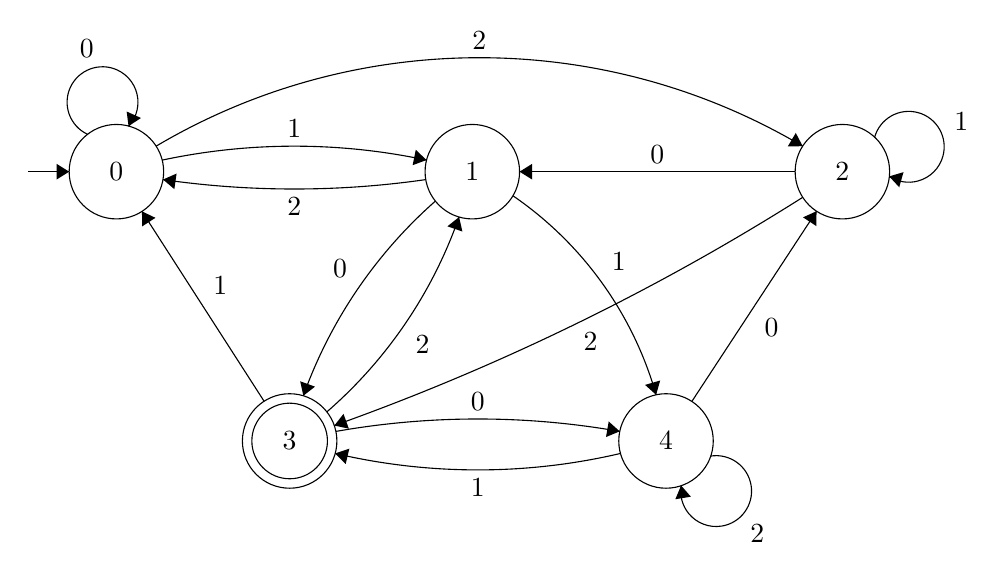
\begin{tikzpicture}[scale=0.2]
    \tikzstyle{every node}+=[inner sep=0pt]
    \draw [black] (9.8,-11.1) circle (3);
    \draw (9.8,-11.1) node {$0$};
    \draw [black] (32.4,-11.1) circle (3);
    \draw (32.4,-11.1) node {$1$};
    \draw [black] (55.9,-11.1) circle (3);
    \draw (55.9,-11.1) node {$2$};
    \draw [black] (44.7,-28.2) circle (3);
    \draw (44.7,-28.2) node {$4$};
    \draw [black] (20.8,-28.2) circle (3);
    \draw (20.8,-28.2) node {$3$};
    \draw [black] (20.8,-28.2) circle (2.4);
    \draw [black] (4.2,-11.1) -- (6.8,-11.1);
    \fill [black] (6.8,-11.1) -- (6,-10.6) -- (6,-11.6);
    \draw [black] (7.978,-8.732) arc (245.30993:-42.69007:2.25);
    \draw (7.92,-3.89) node [above] {$0$};
    \fill [black] (10.57,-8.21) -- (11.36,-7.69) -- (10.45,-7.28);
    \draw [black] (12.323,-9.478) arc (120.60737:59.39263:40.316);
    \fill [black] (53.38,-9.48) -- (52.94,-8.64) -- (52.43,-9.5);
    \draw (32.85,-3.36) node [above] {$2$};
    \draw [black] (12.708,-10.365) arc (102.05097:77.94903:40.196);
    \fill [black] (29.49,-10.36) -- (28.81,-9.71) -- (28.61,-10.69);
    \draw (21.1,-8.98) node [above] {$1$};
    \draw [black] (52.9,-11.1) -- (35.4,-11.1);
    \fill [black] (35.4,-11.1) -- (36.2,-11.6) -- (36.2,-10.6);
    \draw (44.15,-10.6) node [above] {$0$};
    \draw [black] (29.443,-11.603) arc (-81.80808:-98.19192:58.551);
    \fill [black] (12.76,-11.6) -- (13.48,-12.21) -- (13.62,-11.22);
    \draw (21.1,-12.7) node [below] {$2$};
    \draw [black] (19.18,-25.68) -- (11.42,-13.62);
    \fill [black] (11.42,-13.62) -- (11.44,-14.57) -- (12.28,-14.03);
    \draw (15.92,-18.34) node [right] {$1$};
    \draw [black] (31.557,-13.978) arc (-19.27323:-49.02977:29.12);
    \fill [black] (31.56,-13.98) -- (30.82,-14.57) -- (31.77,-14.9);
    \draw (28.77,-22.06) node [right] {$2$};
    \draw [black] (21.668,-25.33) arc (160.29798:131.39902:29.932);
    \fill [black] (21.67,-25.33) -- (22.41,-24.75) -- (21.47,-24.41);
    \draw (24.47,-17.27) node [left] {$0$};
    \draw [black] (23.738,-27.593) arc (100.00912:79.99088:51.853);
    \fill [black] (41.76,-27.59) -- (41.06,-26.96) -- (40.89,-27.95);
    \draw (32.75,-26.3) node [above] {$0$};
    \draw [black] (41.807,-28.993) arc (-76.83063:-103.16937:39.755);
    \fill [black] (23.69,-28.99) -- (24.36,-29.66) -- (24.59,-28.69);
    \draw (32.75,-30.54) node [below] {$1$};
    \draw [black] (47.53,-29.16) arc (99:-189:2.25);
    \draw (50.5,-33.45) node [below] {$2$};
    \fill [black] (45.66,-31.03) -- (45.29,-31.9) -- (46.28,-31.74);
    \draw [black] (46.34,-25.69) -- (54.26,-13.61);
    \fill [black] (54.26,-13.61) -- (53.4,-14) -- (54.24,-14.55);
    \draw (50.92,-20.97) node [right] {$0$};
    \draw [black] (57.945,-8.921) arc (164.55605:-123.44395:2.25);
    \draw (62.98,-7.91) node [right] {$1$};
    \fill [black] (58.87,-11.4) -- (59.51,-12.09) -- (59.78,-11.13);
    \draw [black] (53.381,-12.729) arc (-57.68639:-70.36482:149.833);
    \fill [black] (23.64,-27.22) -- (24.56,-27.42) -- (24.22,-26.48);
    \draw (39.9,-21.3) node [below] {$2$};
    \draw [black] (34.978,-12.629) arc (55.57934:15.87546:22.925);
    \fill [black] (44.07,-25.27) -- (44.33,-24.36) -- (43.37,-24.64);
    \draw (41.22,-16.78) node [right] {$1$};
    \end{tikzpicture}
    \end{center}

\end{enumerate}

\end{document}
